\chapter{METODOLOGI PENELITIAN}

\section{\textit{Proposed Method}}

Penelitian ini mengusulkan metodologi pengembangan sistem pelacakan \textit{invoice} dan \textit{Proof of Delivery} (POD) yang dipadukan dengan rekomendasi prioritas berbasis pengetahuan dan data. Fokus metodologi tidak hanya terletak pada pembangunan aplikasi, tetapi pada proses transformasi pengetahuan operasional menjadi model keputusan yang dapat diuji secara ilmiah. Oleh karena itu, penelitian ini membandingkan pendekatan \textit{knowledge-driven} melalui \textit{Rule-Based System} dan pendekatan \textit{data-driven} melalui Decision Tree C4.5.

\begin{figure}[htbp]
    \centering
    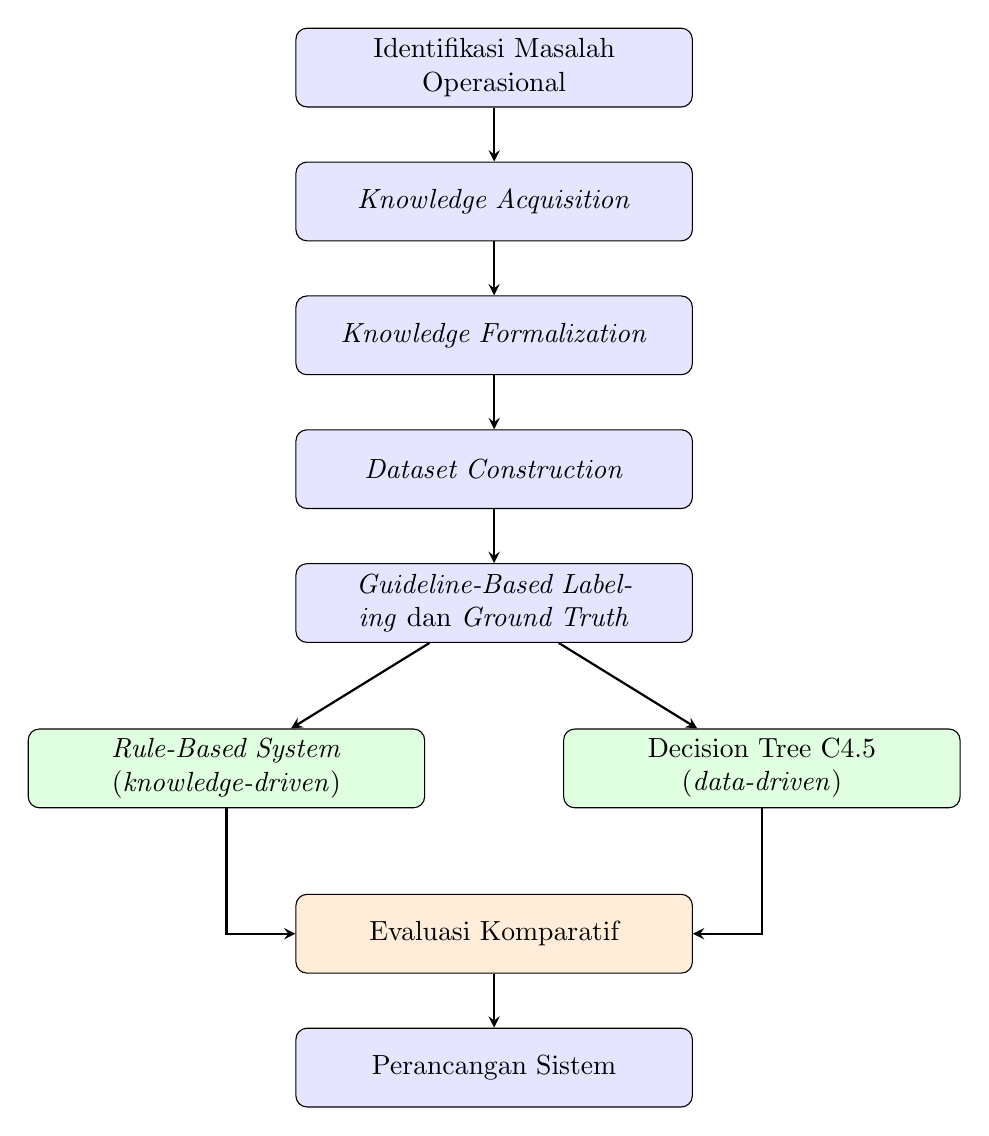
\begin{tikzpicture}[
        block/.style={rectangle, draw=black, fill=blue!10, text width=4.8cm, minimum height=1cm, align=center, rounded corners},
        model/.style={rectangle, draw=black, fill=green!12, text width=4.8cm, minimum height=1cm, align=center, rounded corners},
        eval/.style={rectangle, draw=black, fill=orange!15, text width=4.8cm, minimum height=1cm, align=center, rounded corners},
        arrow/.style={thick, ->, >=stealth}
    ]
        \node[block] (problem) at (0,0) {Identifikasi Masalah Operasional};
        \node[block] (acquisition) at (0,-1.7) {\textit{Knowledge Acquisition}};
        \node[block] (formalization) at (0,-3.4) {\textit{Knowledge Formalization}};
        \node[block] (dataset) at (0,-5.1) {\textit{Dataset Construction}};
        \node[block] (labeling) at (0,-6.8) {\textit{Guideline-Based Labeling} dan \textit{Ground Truth}};
        \node[model] (rule) at (-3.4,-8.9) {\textit{Rule-Based System}\\(\textit{knowledge-driven})};
        \node[model] (tree) at (3.4,-8.9) {Decision Tree C4.5\\(\textit{data-driven})};
        \node[eval] (evaluation) at (0,-11.0) {Evaluasi Komparatif};
        \node[block] (design) at (0,-12.7) {Perancangan Sistem};

        \draw[arrow] (problem) -- (acquisition);
        \draw[arrow] (acquisition) -- (formalization);
        \draw[arrow] (formalization) -- (dataset);
        \draw[arrow] (dataset) -- (labeling);
        \draw[arrow] (labeling) -- (rule);
        \draw[arrow] (labeling) -- (tree);
        \draw[arrow] (rule) |- (evaluation);
        \draw[arrow] (tree) |- (evaluation);
        \draw[arrow] (evaluation) -- (design);
    \end{tikzpicture}
    \caption{Kerangka penelitian}
    \label{fig:kerangka_penelitian}
\end{figure}

Kerangka penelitian pada Gambar \ref{fig:kerangka_penelitian} menunjukkan bahwa masukan utama penelitian berupa masalah keterlambatan dan ketidakterlacakan dokumen \textit{invoice}, regulasi penerimaan pelanggan, data historis \textit{invoice}, serta pengetahuan operasional administrasi. Proses penelitian dilakukan melalui akuisisi pengetahuan, formalisasi pengetahuan, pembentukan dataset, pelabelan berbasis pedoman, pemodelan keputusan, dan evaluasi komparatif. Keluaran dari metodologi ini adalah \textit{ground truth} prioritas, model \textit{Rule-Based}, model Decision Tree C4.5, hasil rancangan sistem, serta dasar evaluasi yang digunakan pada bab hasil dan pembahasan.

\section{\textit{Knowledge Acquisition}}

\textit{Knowledge acquisition} dilakukan untuk memperoleh pengetahuan operasional yang menjadi dasar pembentukan model keputusan prioritas pengiriman \textit{invoice}. Masukan pada tahap ini terdiri atas regulasi pelanggan, data historis \textit{invoice}, dan pengetahuan operasional administrasi. Proses akuisisi dilakukan dengan mengidentifikasi aturan penerimaan dokumen, batas \textit{cut-off}, jadwal penerimaan, serta pertimbangan operasional yang digunakan staf ketika menentukan dokumen mana yang perlu diprioritaskan. Keluaran dari tahap ini adalah kumpulan pengetahuan awal yang masih bersifat tekstual, prosedural, dan sebagian masih berupa \textit{tacit knowledge}.

\begin{table}[htbp]
    \centering
    \small
    \caption{Sumber pengetahuan operasional}
    \label{tab:sumber_pengetahuan}
    \renewcommand{\arraystretch}{1.3}
    \begin{tabularx}{\textwidth}{|>{\raggedright\arraybackslash}p{3.4cm}|>{\raggedright\arraybackslash}X|>{\raggedright\arraybackslash}X|}
        \hline
        \textbf{Sumber Pengetahuan} & \textbf{Bentuk Data} & \textbf{Peran dalam Penelitian} \\ \hline
        Regulasi pelanggan & Aturan \textit{cut-off}, hari penerimaan, dan ketentuan penyerahan dokumen & Menjadi dasar identifikasi batas waktu dan jadwal penerimaan \textit{invoice}. \\ \hline
        Data historis \textit{invoice} & Data pelanggan, tanggal penerimaan, tanggal pengiriman, dan informasi administratif \textit{invoice} & Menjadi dasar pembentukan dataset penelitian dan ekstraksi fitur operasional. \\ \hline
        Pengetahuan operasional administrasi & Pertimbangan staf administrasi dalam menentukan urgensi pengiriman dokumen & Menjadi dasar penyusunan \textit{Operational Labeling Guideline} dan \textit{ground truth}. \\ \hline
    \end{tabularx}
\end{table}

Tahap ini menempatkan staf administrasi dan regulasi pelanggan sebagai sumber pengetahuan domain. Pengetahuan yang diperoleh belum langsung digunakan sebagai aturan keputusan, karena masih perlu diformalkan agar dapat direpresentasikan sebagai atribut dataset dan dipakai secara konsisten oleh dua pendekatan pemodelan yang dibandingkan.

\section{\textit{Knowledge Formalization}}

\textit{Knowledge formalization} merupakan tahap utama dalam penelitian ini karena mengubah pengetahuan operasional yang bersifat implisit menjadi representasi eksplisit. Pengetahuan seperti ``akhir bulan'', ``maksimal tanggal tertentu'', atau ``penerimaan hanya pada hari tertentu'' pada awalnya berbentuk bahasa alami dan belum dapat langsung diproses oleh model keputusan. Tahap formalisasi mengubah pengetahuan tersebut menjadi aturan bisnis, atribut operasional, dan fitur dataset.

\[
\begin{array}{c}
\text{Bahasa alami (natural language)}\\
\downarrow\\
\text{Aturan bisnis (business rule)}\\
\downarrow\\
\text{Atribut operasional}\\
\downarrow\\
\text{Fitur dataset}
\end{array}
\]

Masukan pada tahap ini adalah pengetahuan hasil akuisisi, sedangkan prosesnya berupa penafsiran istilah operasional menjadi struktur atribut yang konsisten. Keluaran tahap ini berupa definisi fitur seperti \texttt{cutoff\_rule}, \texttt{cutoff\_value}, \texttt{receive\_day\_code}, \texttt{days\_to\_cutoff}, \texttt{missed\_receive\_schedule}, dan \texttt{month\_end\_flag}. Dengan proses ini, pengetahuan yang semula bergantung pada interpretasi staf dapat digunakan sebagai dasar model \textit{Rule-Based} dan sebagai fitur pada model Decision Tree C4.5.

\begin{table}[htbp]
    \centering
    \small
    \caption{Contoh formalisasi pengetahuan operasional}
    \label{tab:formalisasi_pengetahuan}
    \renewcommand{\arraystretch}{1.3}
    \begin{tabularx}{\textwidth}{|>{\raggedright\arraybackslash}p{3.2cm}|>{\raggedright\arraybackslash}X|>{\raggedright\arraybackslash}X|}
        \hline
        \textbf{Pengetahuan} & \textbf{Aturan Bisnis} & \textbf{Atribut Formal} \\ \hline
        Akhir bulan & Dokumen pelanggan perlu memperhatikan periode penutupan administrasi bulanan. & \texttt{cutoff\_rule} = \texttt{END\_MONTH}; \texttt{month\_end\_flag}. \\ \hline
        Selasa dan Kamis & Dokumen hanya dapat diterima pada hari penerimaan yang ditentukan pelanggan. & \texttt{receive\_schedule}; \texttt{receive\_day\_code}; \texttt{receive\_days}. \\ \hline
        Maksimal tanggal 10 & Dokumen diterima paling lambat tanggal 10 pada periode berjalan. & \texttt{cutoff\_rule} = \texttt{MONTHLY\_DATE}; \texttt{cutoff\_value} = 10. \\ \hline
        Tanpa \textit{cut-off} & Pelanggan tidak memiliki batas tanggal administratif khusus untuk penerimaan dokumen. & \texttt{cutoff\_rule} = \texttt{NO\_CUTOFF}; \texttt{days\_to\_cutoff} = 999. \\ \hline
    \end{tabularx}
\end{table}

\section{\textit{Dataset Construction}}

\textit{Dataset construction} dilakukan untuk membentuk dataset penelitian setelah pengetahuan operasional diformalkan. Masukan tahap ini adalah data historis \textit{invoice}, data pelanggan, aturan \textit{cut-off}, jadwal penerimaan dokumen, dan atribut hasil formalisasi. Proses konstruksi dataset meliputi integrasi data, ekstraksi fitur, rekayasa fitur, pembersihan nilai yang tidak konsisten, serta penyusunan data akhir yang dapat digunakan untuk pelabelan dan pemodelan.

Integrasi data dilakukan dengan menghubungkan informasi \textit{invoice} dengan regulasi pelanggan. Ekstraksi fitur dilakukan untuk mengambil atribut dasar seperti pelanggan, tanggal penerimaan, aturan \textit{cut-off}, nilai \textit{cut-off}, dan jadwal penerimaan. Rekayasa fitur dilakukan untuk menghasilkan atribut turunan seperti selisih hari menuju \textit{cut-off}, jarak menuju jadwal penerimaan berikutnya, indikator jadwal yang terlewat, dan indikator akhir bulan. Keluaran tahap ini adalah dataset penelitian terstruktur yang memuat fitur operasional dan kolom label prioritas yang akan diisi melalui \textit{Guideline-Based Labeling}.

\begin{table}[htbp]
    \centering
    \small
    \caption{Fitur pada dataset penelitian}
    \label{tab:fitur_dataset}
    \renewcommand{\arraystretch}{1.3}
    \begin{tabularx}{\textwidth}{|>{\raggedright\arraybackslash}p{3.5cm}|>{\raggedright\arraybackslash}p{2.8cm}|>{\raggedright\arraybackslash}X|}
        \hline
        \textbf{Fitur} & \textbf{Tipe} & \textbf{Deskripsi} \\ \hline
        \texttt{customer\_name} atau \texttt{customer\_name\_masking} & Kategorikal & Identitas pelanggan atau identitas pelanggan yang telah disamarkan. \\ \hline
        \texttt{receive\_date} & Tanggal & Tanggal penerimaan atau pencatatan \textit{invoice} sebagai dasar observasi. \\ \hline
        \texttt{cutoff\_type} & Kategorikal & Bentuk aturan \textit{cut-off} pelanggan dalam deskripsi operasional. \\ \hline
        \texttt{cutoff\_value} & Numerik & Nilai tanggal atau batas administratif yang diperoleh dari aturan \textit{cut-off}. \\ \hline
        \texttt{receive\_schedule} & Kategorikal & Deskripsi jadwal penerimaan dokumen, misalnya setiap hari atau hari tertentu. \\ \hline
        \texttt{receive\_day\_code} & Kategorikal & Representasi kode hari penerimaan yang digunakan untuk pemrosesan data. \\ \hline
        \texttt{days\_to\_cutoff} & Numerik & Selisih hari antara tanggal observasi dan batas \textit{cut-off} pelanggan. \\ \hline
        \texttt{next\_receive\_day\_gap} & Numerik & Jarak hari menuju jadwal penerimaan dokumen berikutnya apabila aturan hari penerimaan tersedia. \\ \hline
        \texttt{missed\_receive\_schedule} & Kategorikal & Indikator apakah dokumen telah melewati jadwal penerimaan pelanggan. \\ \hline
        \texttt{month\_end\_flag} & Kategorikal & Indikator apakah dokumen berada pada kondisi akhir bulan yang relevan terhadap prioritas. \\ \hline
        \texttt{final\_label} & Kategorikal & Label prioritas yang dihasilkan melalui \textit{Operational Labeling Guideline} dan digunakan sebagai \textit{ground truth}. \\ \hline
    \end{tabularx}
\end{table}

\section{\textit{Guideline-Based Labeling}}

\textit{Guideline-Based Labeling} bertujuan membentuk \textit{ground truth} prioritas pengiriman \textit{invoice}. Masukan tahap ini adalah dataset penelitian yang telah memuat atribut hasil formalisasi. Proses pelabelan dilakukan dengan menerapkan \textit{Operational Labeling Guideline} yang disusun dari regulasi pelanggan, risiko keterlambatan \textit{cut-off}, keterbatasan hari penerimaan, dan konsekuensi administratif dari keterlambatan dokumen. Keluaran tahap ini adalah label prioritas yang merepresentasikan pedoman keputusan operasional yang telah diformalkan.

Pedoman pelabelan disusun agar proses pemberian label konsisten dan dapat ditelusuri. Label HIGH menunjukkan dokumen yang perlu diprioritaskan karena memiliki risiko administratif tinggi. Label MEDIUM menunjukkan dokumen yang perlu dipantau karena mulai mendekati batas waktu operasional. Label NORMAL menunjukkan dokumen yang belum menunjukkan risiko mendesak atau tidak memiliki batas \textit{cut-off} khusus. Kondisi pelabelan pada Tabel \ref{tab:pedoman_labeling} menggunakan kondisi yang telah didefinisikan dalam penelitian, yaitu kedekatan terhadap \textit{cut-off}, status jadwal penerimaan, kondisi akhir bulan, keterbatasan hari penerimaan, dan kondisi tanpa \textit{cut-off}.

\begin{table}[htbp]
    \centering
    \small
    \caption{Pedoman pelabelan prioritas berbasis operasional}
    \label{tab:pedoman_labeling}
    \renewcommand{\arraystretch}{1.3}
    \begin{tabularx}{\textwidth}{|>{\raggedright\arraybackslash}p{2.5cm}|>{\raggedright\arraybackslash}X|>{\raggedright\arraybackslash}p{3.2cm}|}
        \hline
        \textbf{Label} & \textbf{Kondisi Operasional} & \textbf{Alasan Label} \\ \hline
        HIGH & Dokumen berada pada kondisi \texttt{CUTOFF\_TODAY}, \texttt{OVERDUE\_CUTOFF}, \texttt{CUTOFF\_NEAR}, jadwal penerimaan terbatas (\texttt{LIMITED\_RECEIVE\_DAY}), jadwal penerimaan terlewat, atau kondisi akhir bulan yang dekat dengan \textit{cut-off}. & Risiko keterlambatan tinggi dan perlu diprioritaskan. \\ \hline
        MEDIUM & Dokumen belum memenuhi kondisi HIGH, tetapi berada pada rentang $2 <$ \texttt{days\_to\_cutoff} $\leq 10$ sesuai aturan prioritas yang diformalkan. & Perlu dipantau agar tidak berubah menjadi kondisi mendesak. \\ \hline
        NORMAL & Dokumen memiliki waktu yang masih longgar terhadap \textit{cut-off} (\texttt{LONG\_TIME\_TO\_CUTOFF}) atau berada pada kondisi tanpa \textit{cut-off} khusus (\texttt{NO\_CUTOFF}) tanpa indikasi risiko jadwal penerimaan. & Risiko administratif rendah pada waktu observasi. \\ \hline
    \end{tabularx}
\end{table}

\textit{Ground truth} pada penelitian ini dihasilkan melalui \textit{Operational Labeling Guideline}, bukan oleh model algoritmik. \textit{Ground truth} yang sama digunakan untuk mengevaluasi prediksi \textit{Rule-Based System} dan prediksi Decision Tree C4.5. Dengan demikian, evaluasi kedua pendekatan dilakukan terhadap acuan keputusan yang sama sehingga perbandingan bersifat adil dan terukur.

\section{\textit{Rule-Based Model}}

\textit{Rule-Based Model} merepresentasikan pendekatan \textit{knowledge-driven}, yaitu model keputusan yang dibangun dari pengetahuan operasional dan regulasi pelanggan. Dalam penelitian ini, model berbasis aturan tidak diperlakukan sebagai kode program, melainkan sebagai representasi ilmiah dari pengetahuan operasional yang telah diformalkan. Masukan model adalah atribut hasil \textit{Knowledge Formalization}, yaitu \texttt{cutoff\_rule}, \texttt{days\_to\_cutoff}, \texttt{receive\_schedule}, \texttt{next\_receive\_day\_gap}, \texttt{missed\_receive\_schedule}, dan \texttt{month\_end\_flag}. Keluaran model adalah label prioritas HIGH, MEDIUM, atau NORMAL.

Basis aturan disusun dalam bentuk aturan IF-THEN agar proses pengambilan keputusan dapat ditelusuri secara eksplisit. Setiap aturan memiliki kondisi, label prioritas, dan penjelasan operasional. Apabila lebih dari satu aturan terpenuhi pada data \textit{invoice} yang sama, aturan dengan tingkat prioritas tertinggi digunakan sebagai keputusan akhir dengan urutan HIGH, MEDIUM, kemudian NORMAL. Urutan tersebut digunakan karena risiko keterlambatan administratif pada kelas HIGH lebih kritis dibandingkan kebutuhan pemantauan pada kelas MEDIUM atau kondisi normal.

\begin{table}[htbp]
    \centering
    \scriptsize
    \caption{Rule base penentuan prioritas pengiriman invoice}
    \label{tab:rule_base_priority}
    \renewcommand{\arraystretch}{1.35}
    \begin{tabularx}{\textwidth}{|>{\raggedright\arraybackslash}p{1.1cm}|>{\raggedright\arraybackslash}X|>{\centering\arraybackslash}p{1.8cm}|>{\raggedright\arraybackslash}X|}
        \hline
        \textbf{Rule ID} & \textbf{Condition} & \textbf{Priority} & \textbf{Description} \\ \hline
        R1 &
        \textbf{IF} \texttt{missed\_receive\_schedule} = \textit{Yes} &
        HIGH &
        Jadwal penerimaan dokumen pelanggan telah terlewat, sehingga dokumen berisiko tidak dapat diproses pada periode administrasi berjalan. \\ \hline
        R2 &
        \textbf{IF} \texttt{cutoff\_rule} $\neq$ \texttt{NO\_CUTOFF} \newline
        \textbf{AND} \texttt{days\_to\_cutoff} $< 0$ &
        HIGH &
        Dokumen telah melewati batas \textit{cut-off} pelanggan sehingga diperlukan prioritas tertinggi untuk mengurangi dampak keterlambatan. \\ \hline
        R3 &
        \textbf{IF} \texttt{cutoff\_rule} $\neq$ \texttt{NO\_CUTOFF} \newline
        \textbf{AND} \texttt{days\_to\_cutoff} = 0 &
        HIGH &
        Tanggal observasi bertepatan dengan batas \textit{cut-off}; dokumen harus segera dikirim agar masih dapat diterima pada hari yang sama. \\ \hline
        R4 &
        \textbf{IF} \texttt{cutoff\_rule} $\in$ \{\texttt{END\_MONTH}, \texttt{MONTHLY\_DATE}, \texttt{MULTIPLE\_MONTHLY\_DATE}\} \newline
        \textbf{AND} $0 <$ \texttt{days\_to\_cutoff} $\leq 2$ &
        HIGH &
        Dokumen mendekati batas administratif bulanan atau tanggal bulanan tertentu, sehingga ruang koreksi operasional sangat terbatas. \\ \hline
        R5 &
        \textbf{IF} \texttt{cutoff\_rule} $\in$ \{\texttt{NEXT\_MONTH\_DATE}, \texttt{NEXT\_MONTH\_WORKDAY}, \texttt{NEXT\_MONTH\_FIRST\_WEEK}\} \newline
        \textbf{AND} $0 <$ \texttt{days\_to\_cutoff} $\leq 2$ &
        HIGH &
        Dokumen mendekati batas penerimaan pada awal bulan berikutnya atau batas hari kerja bulan berikutnya. \\ \hline
        R6 &
        \textbf{IF} \texttt{month\_end\_flag} = \textit{Yes} \newline
        \textbf{AND} \texttt{days\_to\_cutoff} $\leq 4$ &
        HIGH &
        Dokumen berada pada periode akhir bulan yang sensitif terhadap penutupan administrasi, sehingga keterlambatan kecil dapat berdampak pada periode tagihan. \\ \hline
        R7 &
        \textbf{IF} \texttt{receive\_schedule} $\neq$ \textit{Everyday} \newline
        \textbf{AND} \texttt{next\_receive\_day\_gap} $\leq 1$ &
        HIGH &
        Pelanggan hanya menerima dokumen pada hari tertentu dan kesempatan penerimaan berikutnya sangat dekat, sehingga dokumen perlu segera diprioritaskan. \\ \hline
        R8 &
        \textbf{IF} \texttt{cutoff\_rule} $\neq$ \texttt{NO\_CUTOFF} \newline
        \textbf{AND} $2 <$ \texttt{days\_to\_cutoff} $\leq 10$ \newline
        \textbf{AND} tidak memenuhi R1--R7 &
        MEDIUM &
        Dokumen belum berada pada kondisi kritis, tetapi mulai mendekati batas administratif sehingga perlu dipantau agar tidak berubah menjadi prioritas tinggi. \\ \hline
        R9 &
        \textbf{IF} \texttt{receive\_schedule} $\neq$ \textit{Everyday} \newline
        \textbf{AND} \texttt{next\_receive\_day\_gap} $> 1$ \newline
        \textbf{AND} tidak memenuhi R1--R7 &
        MEDIUM &
        Jadwal penerimaan pelanggan terbatas, tetapi masih terdapat kesempatan operasional sebelum dokumen masuk kategori mendesak. \\ \hline
        R10 &
        \textbf{IF} \texttt{cutoff\_rule} = \texttt{NO\_CUTOFF} \newline
        \textbf{AND} \texttt{missed\_receive\_schedule} = \textit{No} \newline
        \textbf{AND} tidak terdapat risiko jadwal penerimaan &
        NORMAL &
        Pelanggan tidak memiliki batas \textit{cut-off} khusus dan tidak terdapat indikasi risiko pada jadwal penerimaan dokumen. \\ \hline
        R11 &
        \textbf{IF} \texttt{cutoff\_rule} $\neq$ \texttt{NO\_CUTOFF} \newline
        \textbf{AND} \texttt{days\_to\_cutoff} $> 10$ \newline
        \textbf{AND} tidak memenuhi R1--R9 &
        NORMAL &
        Batas administratif masih relatif jauh sehingga dokumen belum memerlukan perlakuan prioritas khusus. \\ \hline
        R12 &
        \textbf{IF} tidak ada kondisi pada R1--R11 yang terpenuhi &
        NORMAL &
        Aturan penutup digunakan untuk menjaga setiap data \textit{invoice} tetap memperoleh label prioritas yang konsisten. \\ \hline
    \end{tabularx}
\end{table}

Tabel \ref{tab:rule_base_priority} menunjukkan bahwa basis aturan dibentuk dari tiga kelompok pengetahuan utama. Kelompok pertama adalah aturan \textit{cut-off}, yaitu aturan yang memeriksa kedekatan dokumen terhadap batas administratif pelanggan. Kelompok kedua adalah aturan jadwal penerimaan, yaitu aturan yang memeriksa apakah dokumen masih berada dalam jadwal penerimaan yang diperbolehkan. Kelompok ketiga adalah aturan kondisi khusus, seperti akhir bulan, yang dapat meningkatkan tingkat urgensi meskipun batas \textit{cut-off} belum benar-benar jatuh pada hari observasi.

\begin{figure}[htbp]
    \centering
    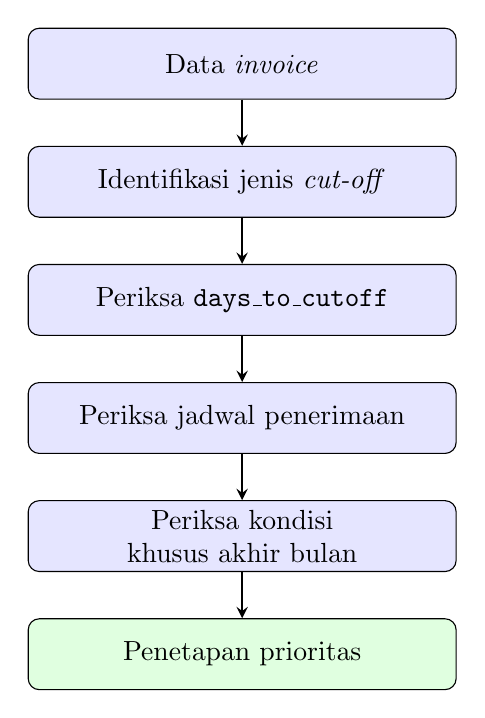
\begin{tikzpicture}[
        block/.style={rectangle, draw=black, fill=blue!10, text width=5.2cm, minimum height=0.9cm, align=center, rounded corners},
        decision/.style={rectangle, draw=black, fill=green!12, text width=5.2cm, minimum height=0.9cm, align=center, rounded corners},
        arrow/.style={thick, ->, >=stealth}
    ]
        \node[block] (invoice) at (0,0) {Data \textit{invoice}};
        \node[block] (cutofftype) at (0,-1.5) {Identifikasi jenis \textit{cut-off}};
        \node[block] (daystocutoff) at (0,-3.0) {Periksa \texttt{days\_to\_cutoff}};
        \node[block] (schedule) at (0,-4.5) {Periksa jadwal penerimaan};
        \node[block] (special) at (0,-6.0) {Periksa kondisi khusus akhir bulan};
        \node[decision] (priority) at (0,-7.5) {Penetapan prioritas};

        \draw[arrow] (invoice) -- (cutofftype);
        \draw[arrow] (cutofftype) -- (daystocutoff);
        \draw[arrow] (daystocutoff) -- (schedule);
        \draw[arrow] (schedule) -- (special);
        \draw[arrow] (special) -- (priority);
    \end{tikzpicture}
    \caption{Rule dependency diagram pada model berbasis aturan}
    \label{fig:rule_dependency_diagram}
\end{figure}

Gambar \ref{fig:rule_dependency_diagram} menggambarkan ketergantungan antaraturan dalam proses penentuan prioritas. Pemeriksaan dimulai dari data \textit{invoice}, kemudian dilanjutkan dengan identifikasi jenis \textit{cut-off}, kedekatan terhadap batas waktu, jadwal penerimaan, serta kondisi khusus akhir bulan. Struktur ini menunjukkan bahwa keputusan prioritas tidak hanya ditentukan oleh satu atribut, tetapi oleh kombinasi pengetahuan administratif pelanggan dan kondisi operasional pada tanggal observasi.

\begin{figure}[htbp]
    \centering
    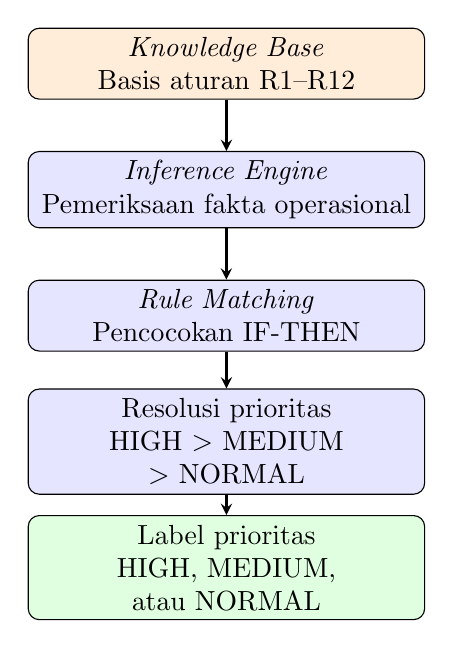
\begin{tikzpicture}[
        block/.style={rectangle, draw=black, fill=orange!15, text width=4.8cm, minimum height=0.9cm, align=center, rounded corners},
        process/.style={rectangle, draw=black, fill=blue!10, text width=4.8cm, minimum height=0.9cm, align=center, rounded corners},
        output/.style={rectangle, draw=black, fill=green!12, text width=4.8cm, minimum height=0.9cm, align=center, rounded corners},
        arrow/.style={thick, ->, >=stealth}
    ]
        \node[block] (kb) at (0,0) {\textit{Knowledge Base}\\Basis aturan R1--R12};
        \node[process] (engine) at (0,-1.6) {\textit{Inference Engine}\\Pemeriksaan fakta operasional};
        \node[process] (matching) at (0,-3.2) {\textit{Rule Matching}\\Pencocokan IF-THEN};
        \node[process] (conflict) at (0,-4.8) {Resolusi prioritas\\HIGH $>$ MEDIUM $>$ NORMAL};
        \node[output] (priority) at (0,-6.4) {Label prioritas\\HIGH, MEDIUM, atau NORMAL};

        \draw[arrow] (kb) -- (engine);
        \draw[arrow] (engine) -- (matching);
        \draw[arrow] (matching) -- (conflict);
        \draw[arrow] (conflict) -- (priority);
    \end{tikzpicture}
    \caption{Rule inference flow pada model berbasis aturan}
    \label{fig:rule_inference_flow}
\end{figure}

Gambar \ref{fig:rule_inference_flow} menunjukkan alur inferensi pada model berbasis aturan. \textit{Knowledge base} menyediakan aturan eksplisit, sedangkan \textit{inference engine} menggunakan fakta operasional pada setiap data \textit{invoice} untuk melakukan pencocokan aturan. Hasil pencocokan kemudian diselesaikan melalui urutan prioritas sehingga keluaran akhir berupa label HIGH, MEDIUM, atau NORMAL. Dengan alur tersebut, setiap keputusan model dapat dijelaskan kembali melalui aturan yang memicunya.

\section{\textit{Decision Tree} C4.5}

Decision Tree C4.5 merepresentasikan pendekatan \textit{data-driven}. Masukan model ini adalah dataset penelitian yang telah memiliki fitur operasional dan label berbasis \textit{Operational Labeling Guideline}. Sebelum pelatihan, fitur kategorikal disiapkan agar dapat diproses oleh model, sedangkan label prioritas digunakan sebagai target pembelajaran. Dataset kemudian dibagi menjadi data latih dan data uji secara terstratifikasi agar proporsi kelas pada proses evaluasi tetap terjaga.

Proses pelatihan dilakukan dengan membentuk pohon keputusan dari data latih. Pemilihan atribut pada setiap node dilakukan berdasarkan pengurangan ketidakpastian kelas, yaitu melalui perhitungan \textit{entropy} dan \textit{information gain}. Atribut dengan kontribusi pemisahan paling informatif dipilih sebagai node, kemudian proses pemisahan berlanjut hingga terbentuk struktur pohon keputusan. Keluaran tahap ini adalah model Decision Tree C4.5 yang menghasilkan prediksi prioritas terhadap data uji.

Penjelasan teori mengenai \textit{entropy} dan \textit{information gain} telah dibahas pada Bab II, sehingga bagian ini hanya menempatkannya sebagai prosedur metodologis. Dalam penelitian ini, konsep tersebut digunakan untuk menghasilkan model pembanding terhadap aturan eksplisit operasional, bukan sebagai pengganti \textit{ground truth} yang telah dibangun melalui \textit{Guideline-Based Labeling}.

\section{\textit{Comparative Evaluation}}

Evaluasi komparatif dilakukan untuk membandingkan kemampuan pendekatan \textit{knowledge-driven} dan \textit{data-driven} dalam merepresentasikan keputusan prioritas berdasarkan pedoman operasional. Masukan evaluasi adalah \textit{ground truth} hasil \textit{Guideline-Based Labeling}, prediksi dari \textit{Rule-Based System}, dan prediksi dari Decision Tree C4.5. Proses evaluasi menggunakan acuan yang sama untuk kedua model agar hasil perbandingan tidak dipengaruhi oleh perbedaan standar penilaian.

\[
\begin{array}{c}
\text{Ground Truth}\\
\downarrow\\
\text{Rule-Based Prediction dan Decision Tree Prediction}\\
\downarrow\\
\text{Confusion Matrix}\\
\downarrow\\
\text{Accuracy, Precision, Recall, F1-score}
\end{array}
\]

\textit{Confusion matrix} digunakan untuk menunjukkan distribusi prediksi benar dan salah pada kelas HIGH, MEDIUM, dan NORMAL. Dari matriks tersebut dihitung \textit{accuracy}, \textit{precision}, \textit{recall}, dan \textit{F1-score}. Keluaran tahap ini bukan nilai hasil eksperimen pada bab metodologi, melainkan rancangan evaluasi yang digunakan untuk menilai kesesuaian kedua pendekatan terhadap \textit{ground truth} pada bab hasil dan pembahasan.

\section{\textit{System Design}}

\textit{System design} ditempatkan setelah metodologi pemodelan karena perancangan perangkat lunak berfungsi sebagai wadah penerapan proses pelacakan \textit{invoice}, penyimpanan POD, dan penyajian hasil prioritas. Masukan tahap ini adalah kebutuhan operasional pengguna, hasil analisis data, dan kebutuhan integrasi model prioritas. Proses perancangan dilakukan melalui arsitektur sistem, Use Case Diagram, Activity Diagram, dan Entity Relationship Diagram (ERD). Keluaran tahap ini adalah rancangan sistem yang menjadi dasar implementasi aplikasi.

\noindent\textbf{Arsitektur sistem.}
Sistem dirancang dengan pendekatan \textit{client-server}. Pengguna mengakses antarmuka web untuk mencatat \textit{invoice}, memperbarui status pengiriman, mengunggah POD, dan melihat prioritas. Server memproses permintaan pengguna, menjalankan logika bisnis, mengakses basis data, dan menyediakan hasil prioritas. Basis data menyimpan data pelanggan, data \textit{invoice}, riwayat pelacakan, dokumen POD, dan catatan prioritas.

\begin{figure}[htbp]
    \centering
    \includegraphics[width=0.95\textwidth]{\detokenize{diagram-blok-arsitektur-sistem.png}}
    \caption{Arsitektur sistem pelacakan invoice dan POD}
    \label{fig:arsitektur_sistem}
\end{figure}

\noindent\textbf{Use Case Diagram.}
Use Case Diagram menggambarkan interaksi aktor dengan sistem. Aktor utama adalah staf administrasi yang mengelola data pelanggan, mencatat \textit{invoice}, memperbarui status pengiriman, mengunggah POD, melihat riwayat pelacakan, dan melihat rekomendasi prioritas. Diagram ini digunakan untuk memastikan kebutuhan fungsional sistem sesuai dengan proses operasional.

\begin{figure}[htbp]
    \centering
    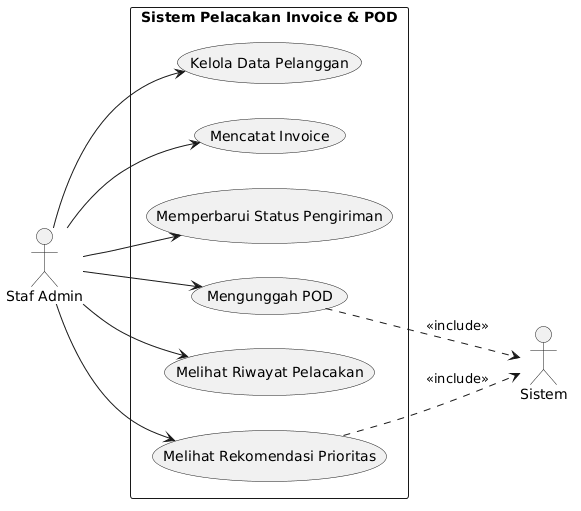
\includegraphics[width=0.8\textwidth]{use-case-diagram.png}
    \caption{Use Case Diagram Sistem Pelacakan Invoice dan POD}
    \label{fig:use_case_diagram}
\end{figure}

\noindent\textbf{Activity Diagram.}
Activity Diagram memodelkan alur kerja unggah POD dan pembaruan status \textit{invoice}. Alur dimulai ketika pengguna memilih data \textit{invoice}, mengunggah bukti penerimaan, dan mengirimkan data ke sistem. Sistem kemudian memvalidasi masukan, menyimpan POD, memperbarui status, dan menambahkan catatan pada riwayat pelacakan.

\begin{figure}[htbp]
    \centering
    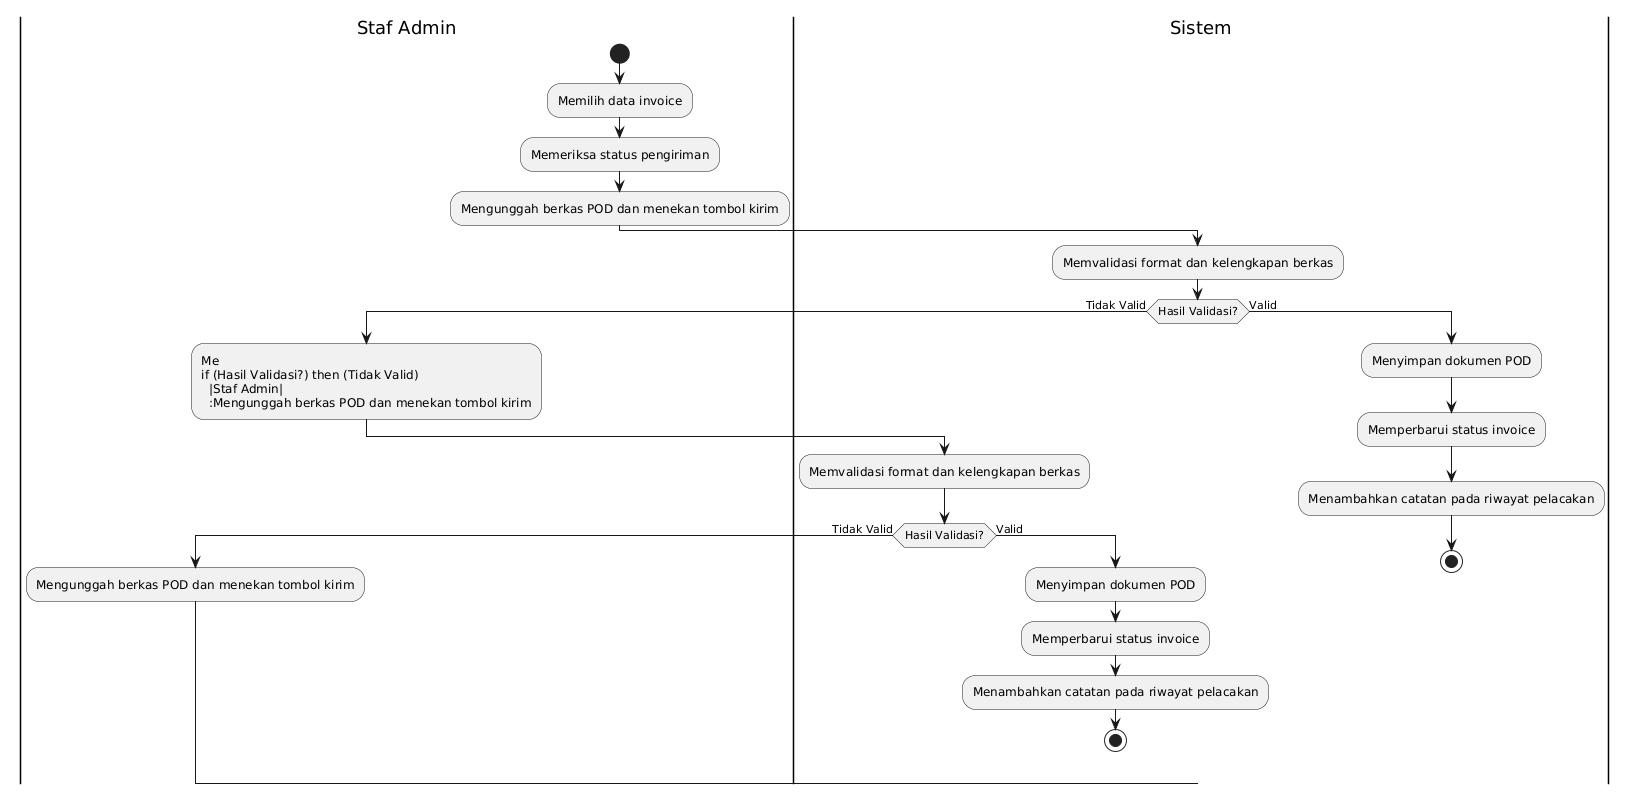
\includegraphics[width=1\textwidth]{activity-diagram.png}
    \caption{Activity Diagram Sistem Pelacakan dan POD}
    \label{fig:activity_pod}
\end{figure}

\noindent\textbf{Entity Relationship Diagram.}
ERD menggambarkan struktur data yang mendukung sistem. Entitas utama meliputi pelanggan, \textit{invoice}, pengiriman atau pelacakan, pengguna, dan catatan prioritas. Relasi antarentitas memastikan setiap \textit{invoice} dapat ditelusuri terhadap pelanggan, status pengiriman, bukti penerimaan, dan hasil prioritas yang terkait.

\begin{figure}[htbp]
    \centering
    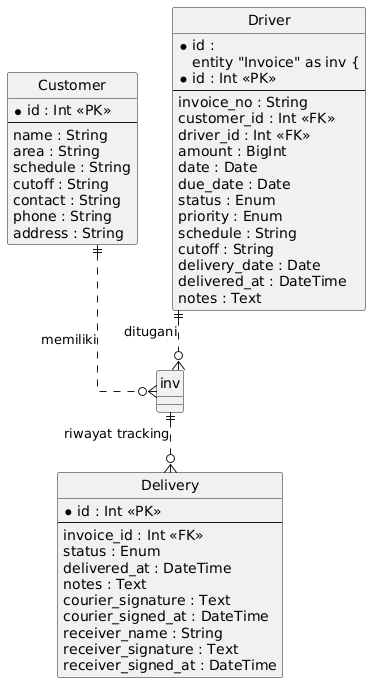
\includegraphics[width=0.8\textwidth]{ERD.png}
    \caption{ERD sistem pelacakan invoice dan POD}
    \label{fig:erd}
\end{figure}
